% Overview:
%   VarGeno TeX subfile for the project.
%   Each subfile MUST start with the following line
%		\documentclass[../main.tex]{subfiles}

\documentclass[../main.tex]{subfiles}

\begin{document}

\subsection{VarGeno}
\label{vargeno}
Volendo analizzare l’attuale stato dell’arte rispetto ai metodi di ricerca e genotipizzazione di SNP senza l'utilizzo dell'allineamento e \textit{reference based}, certamente un framework da presentare e studiare è VarGeno. Nel paper \cite{sun-medvedev2018vargeno}, viene presentato VarGeno, il loro sistema per la genotipizzazione di SNP da dati di sequenziamento dell’intero genoma. Esso si basa su LAVA, lightweight assignment of variant alleles \cite{shajii2016lava}, un precedente algoritmo di genotipizzazione, basato su NGS per un assegnato set di loci SNP, che sfrutta il fatto che, in genere, la corrispondenza approssimativa di k-mer di medie dimensioni è in grado di identificare univocamente i loci nel genoma umano senza un allineamento completo delle read. Partendo da LAVA, che aveva già dichiarato prestazioni 4-7 volte più veloci di una pipeline standard di genotipizzazione basata sull’allineamento, con una precisione comparabile, vengono migliorate la velocità di interrogazione dei k-mer e l'accuratezza della strategia di genotipizzazione, arrivando con VarGeno ad ottenere prestazioni 7–13 volte più veloci di LAVA con un utilizzo di memoria simile e migliorando allo stesso tempo la precisione.

VarGeno introduce una differente struttura dati utile per indicizzare e interrogare i k-mer, i Bloom filter (vedi sezione \ref{BloomFilter}), e nella maggioranza delle condizioni utilizza la scansione lineare oer la ricerca all'interno di blocchi. Inoltre, nella fase finale, quella in cui avviene la genotipizzazione, vengono utilizzati i valori di qualità e impiegati diversi criteri di mappatura per migliorare la velocità e l'accuratezza. 

Possiamo affermare che l’algoritmo di base di VarGeno può essere visto come l’insieme di queste componenti: l’algoritmo di base di LAVA, l’uso dei Bloom Filter, la scansione lineare, un cutoff dato dai valori di qualità e nuovi criteri di mappatura delle read. Inizieremo quindi con l’introdurre l’algoritmo di LAVA; seguirà un paragrafo per presentare i Bloom Filter e il loro funzionamento di base, per poi discutere di tutte le modifiche apportate a LAVA per ricostruire l’intero algoritmo di VarGeno. Viene presentato l'approccio di LAVA poichè costituisce un rilevante punto di partenza: alcune delle sue componenti verranno infatti riprese anche da altri framework che tratteremo in seguito.

\subsubsection{Algoritmo di LAVA}
LAVA (lightweight assignment of variant alleles), è un framework che crea degli indici dalla lista in input di SNP noti (ad es. dbSNP) e dalla sequenza di riferimento e utilizza poi una corrispondenza approssimativa dei k-mer per genotipizzare il donatore dai dati di sequenziamento, usando le read grezze e non ancora elaborate.
  
Il framework prende in input il genoma di riferimento, una lista di SNP e un set di read e restituisce in output i genotipi predetti per gli SNP. 

In particolare, data una lista di SNP, costruisce un dizionario completo di k-mer (con k = 32) che identificano in modo univoco quegli SNP (ove possibile). Abbinata ad un secondo dizionario di tutti i k-mer nel genoma di riferimento, è in grado di determinare rapidamente se una read appartiene a un particolare SNP come allele selvatico (\textit{wild-type}) o allele mutato, attraverso una corrispondenza bipartita di k-mer nelle read con i k-mer nei dizionari precompilati, fino ad una distanza di Hamming uguale a 1; non viene eseguito perciò nessun allineamento delle read. Aggregando le read rilevanti, LAVA definisce gli SNP con un modello probabilistico usando la coverage prevista delle read e la frequenza a priori delle varianti nella lista di SNP.\\

L’algoritmo usa come lunghezza di base dei k-mer, k = 32, per una serie di motivi che elenchiamo; dobbiamo evidenziare che, per gli stessi motivi, anche successivamente VarGeno utilizzerà questo valore per questo parametro. Osserviamo che i k-mer dovrebbero identificare in modo univoco i luoghi del genoma in cui si trovano gli SNP di interesse. La lunghezza scelta innanzitutto è adatta per rappresentare nelle attuali macchine i k-mer, che possono semplicemente essere codificati come numeri a 64 bit; tenendo inoltre conto dei possibili errori, k dovrebbe essere sufficientemente lungo per evitare che i k-mer abbiano vicini di Hamming nel genoma (loci che si trovano a una distanza di Hamming 1). \cite{shajii2016lava} mostrano come scegliendo k = 32, siamo in grado di localizzare in modo univoco l'85,7\% del genoma umano con corrispondenze esatte a 32-mer e il 79,3\% considerando anche i vicini di Hamming a distanza 1. Scegliendo k inferiore la percentuale diminuisce quindi non è conveniente ma, anche se aumentando k la proporzione di loci univocamente identificabili aumenta, k = 32 sembra aver superato un punto di flesso e l'aumento non è considerevole. Un k troppo elevato inoltre richiederebbe troppa memoria e comporterebbe un aumento della possibilità di errori di sequenziamento: l’algoritmo controlla anche i vicini di Hamming a distanza 1, correggendo un singolo errore, ma guardare a distanze più alte richiederebbe esponenzialmente più tempo. Scegliendo k = 32, si garantisce che raramente i k-mer abbiano più di un errore.\\

Dopo aver chiarito questa scelta, procediamo con l’effettivo algoritmo. Nella fase di \textit{preprocessing}, l’algoritmo lavora sulla sequenza di riferimento, considerando ogni sottostringa di lunghezza k che appare al suo interno, con l’obiettivo di creare un dizionario, $D_{ref}$, che associa ciascun k-mer all'indice nella sequenza del genoma di riferimento in cui esso appare (se appare più di una volta, vengono memorizzate più posizioni, fino ad un massimo di 9). $D_{ref}$ può essere trattato come un elenco di tuple <k-mer, indice>, in cui il k-mer è rappresentato dalla sua codifica intera senza segno a 64 bit; per ottimizzare la ricerca, le tuple vengono ordinate secondo i valori dei k-mer codificati e viene utilizzata una hash table, $J_{ref}$, che associa ogni intero senza segno a 32 bit \textit{u} alla prima posizione in $D_{ref}$ in cui c’è un 32-mer i cui 32 bit superiori della codifica coincidono con \textit{u}. Poiché $D_{ref}$ è ordinato in base ai valori numerici dei 32-mer codificati, i 32-mer le cui codifiche hanno gli stessi 32 bit superiori sono raggruppati in un bucket ordinato, diminuendo gli errori e facilitando la ricerca di tutti i vicini di Hamming di un k-mer: per effettuare la ricerca di un k-mer in $D_{ref}$ viene individuata la posizione di partenza del bucket a cui appartiene, usando $J_{ref}$ (cercando la corrispondenza con i 32 bit superiori) e la posizione di partenza del bucket successivo (la posizione a cui punta il successivo elemento in $J_{ref}$) e viene eseguita una ricerca binaria nel bucket.

Per quanto riguarda la lista di SNP data in input, ogni suo elemento è costituito dalla posizione nel riferimento in cui si trova, l’allele di riferimento, l’allele alternato e frequenze a priori degli alleli nella popolazione. Essa è pre-elaborata in modo analogo alla sequenza del genoma di riferimento: si costruisce un dizionario indice in cui vengono inseriti non tutti i k-mer ma solamente quelli che si sovrappongono ad alcuni SNP con l'allele alternato al posto dell’allele di riferimento. Il dizionario creato $D_{SNP}$ (così come la hash table $J_{SNP}$) contiene i k-mer con l'allele mutante e, oltre alle posizioni, include le informazioni sugli SNP. 
Per quanto riguarda la complessità di spazio delle strutture dati presentate, esse hanno dimensioni al massimo lineari nella taglia del genoma, perché ogni locus nel genoma e ciascun SNP contribuiscono con un k-mer e ogni k-mer non memorizza più di informazioni costanti.\\

Riguardo all’elaborazione online delle read, al fine di determinarne le varianti, viene creata una \textit{pileup table}, P, in cui vengono memorizzati, per ogni SNP, i conteggi dell'allele di riferimento e dell'allele alternato ($\alpha$ e $\beta$ rispettivamente), che vengono aggiornati in modo incrementale durante l'elaborazione. La tabella può essere implementata per usare spazio lineare nella lunghezza del genoma o, usando una hash table, nel numero di SNP, quindi la complessità in spazio di LAVA è determinata dalle strutture statiche della fase di pre-processing.

L'elaborazione di una read inizia con la sua divisione in k-mer contigui e non sovrapposti: l’obiettivo è determinare quale SNP, se presente, corrisponde alla lettura. Gli SNP vengono identificati interrogando i dizionari $D_{ref}$ e $D_{SNP}$, per ogni k-mer campionato dalla read, con tutti i k-mer a distanza di Hamming 1. Quindi, per ogni read, si identifica quale locus il maggior numero di k-mer in quella read corrisponde. Se c’è più di un locus o se non ce n’è nessuno supportato da due o più k-mer, P non viene aggiornata. Quando la procedura è stata applicata a tutte le read e la tabella P è compilata con i conteggi, l’ultimo passo è la determinazione degli SNP, che sfrutta un modello probabilistico: questo step è comune a molti altri framework, che nella loro fase finale sfruttano le probabilità per chiamare il genotipo. Viene assegnata un'etichetta ``omozigote di riferimento", ``eterozigote" o ``omozigote alternato" a ciascuna posizione in P, coperta da almeno una read poiché, avendo le frequenze degli alleli di riferimento e alternati, si può stimare la probabilità a posteriori di ogni genotipo, usando la regola di Bayes. Si determina come genotipo quello che ha la maggiore probabilità, dato l’evento osservato. \\

LAVA ottiene elevate prestazioni rispetto agli altri algoritmi standard che utilizzano l’allineamento, migliorando i tempi di esecuzione di un fattore 4-7 e mantenendo una elevata accuratezza (93.1\% sulla lista dbSNP e 96.4\% sulla lista Affymetrix SNP Array 6.0, ma rispettivamente 98.5\% e 97.9\% sulle chiamate tentate, dato che non tutti gli SNP possono essere identificati univocamente da uno dei loro 32-mer sovrapposti).
Il framework LAVA si concentra sugli SNP ma è fattibile, secondo gli autori in  \cite{shajii2016lava}, pensare di estenderlo ed utilizzarlo anche per altre mutazioni, come piccoli indel (inserzioni e delezioni) o CNV (Copy Number Variation). Inoltre, una volta eseguita la fase di confronto dei k-mer, è possibile applicare un numero qualsiasi di diversi modelli probabilistici per chiamarre la base e determinare la più probabile. 

\subsubsection{Bloom Filter}
\label{BloomFilter}
Un Bloom filter è una struttura dati probabilistica efficiente in termini di spazio, creata per migliorare la scalabilità \cite{sun-medvedev2018vargeno}. Per la loro semplicità ed efficacia sono usati per molteplici problemi in bioinformatica, come la rappresentazione dei grafi di \textit{Bruijn} (che tratteremo in seguito) e il conteggio di k-mer in un campione. Il Bloom filter rappresenta fondamentalmente un insieme di elementi e consente di effettuare query di appartenenza approssimative, per determinare cioè se un elemento appartiene o no all'insieme dei dati del Bloom filter. Il risultato di tali query può essere un falso positivo ma mai un falso negativo: questo significa che il filtro può verificare se un valore è ``possibilmente nel set" (ci possono essere casi in cui si pensa erroneamente che l'elemento appartenga) o ``sicuramente non nel set"; è chiamato struttura dati \textit{probabilistica} proprio per questo motivo. Esso è molto efficiente in termini di spazio poichè, quando una tabella hash richiede di avere dimensioni arbitrarie in base ai dati di input, esso funziona bene con una dimensione fissa.


\theoremstyle{definition}
\begin{definition} 

Un Bloom filter, che rappresenta un insieme di elementi \textit{S} di cardinalità \textit{n}, è un vettore di bit di lunghezza \textit{m} e un insieme di \textit{h} funzioni di hash \{$H_{1}$, ... , $H_{h}$\}, ognuna delle quali mappa ogni elemento in un valore indice \{1, ... , \textit{m}\}. 

\end{definition}

Inizialmente tutti i bit del vettore sono impostati a 0. Quando un elemento \textit{e} viene aggiunto all'insieme, vengono impostati a 1 gli elementi delle celle di indice \{$H_{1}(e)$, ... , $H_{h}(e)$\}. Per verificare che un elemento appartenga all'insieme significa controllare che tutte le posizioni \{$H_{1}(e)$, ... , $H_{h}(e)$\} siano 1: se anche una sola posizione è settata a 0, questo significa che l'elemento sicuramente non è nel set, altrimenti, se tutte le posizioni contengono il bit 1, allora probabilmente l'elemento appartiene \cite{compressedbloomfilter}. Il \textit{probabilmente} è dovuto al fatto che le celle potrebbero essere state settate a 1 a causa dell'inserimento di altri elementi, poichè le funzioni hash collidono. Si intuisce che quindi sono solo due le operazioni supportate dai Bloom filter, l'inserimento e il test per verificare l'appartenenza: l'operazione di rimozione non è supportata dalla versione standard, poichè settando a 0 tutti i bit presenti nelle posizioni relative alle funzioni di hash potrebbe annullare anche l'effetto dell'inserimento di altri elementi, le cui alcune funzioni di hash collidevano. In una possibile variante in cui si richiede di supportare la rimozione, chiamata \textit{Counting bloom filter}, si può pensare di memorizzare nelle varie posizioni un valore intero (e non solo bit): invece di contrassegnare il bit su "1" quando si inserisce un valore, si aumenta il valore intero di una unità; quando invece un elemento viene rimosso, il valore corrispettivo alle posizioni date dalle funzioni di hash viene ridotto di una unità. Per verificare l'esistenza di un elemento si controlla se gli indici corrispondenti alle funzioni hash contengono un valore maggiore di 0. Questa modifica al fine di supportare la funzionalità di rimozione, aumenta le dimensioni e comporta l'uso di più spazio. L'operazione di rimozione non è invece richiesta nelle applicazioni presentate in questo paper.

Concentrandoci sull'aspetto dei falsi positivi, possiamo dimostrare che la probabilità che si verifichino è sufficientemente bassa. Dato un Bloom filter di un set di \textit{n} elementi, con \textit{h} funzioni di hash e un vettore di \textit{m} bit è $(1 - e^{\frac{-hn}{m}})^{h} $; pertanto, aumentando le dimensioni del filtro si riduce la percentuale di falsi positivi \cite{bernardini2019malva} \cite{compressedbloomfilter}. Se la dimensione è troppo piccola, i campi si riempiranno velocemente e la percentuale di falsi positivi sarà molto alta, ma si riduce l'utilizzo della memoria. 

Un altro parametro importante è il numero di funzioni hash utilizzate. In generale, più funzioni hash vengono usate, più lento sarà il filtro bloom e più velocemente si riempirà ma la percentuale di falsi positivi sarà limitata; se ce ne sono troppo poche, tuttavia, potrebbero esserci troppo falsi positivi.\\

L'\textit{One-Hashing Bloom Filter} (OHBF), è una variante dei Bloom filter che ha lo scopo di abbassare il costo di calcolo che altrimenti potrebbe limitare le prestazioni: richiede solo una funzione hash di base più altre semplici operazioni. Pur mantenendo quasi lo stesso rapporto teorico di falsi positivi di un filtro Bloom standard, l'OHBF riduce significativamente il sovraccarico di calcolo dell'hash \cite{bloomonehash}. Questo risulta in un approccio molto efficiente con un confermato limite alle prestazioni. In \cite{bloomonehash} dimostrano che l'uso di molteplici buone funzioni di hash non porta necessariamente a migliori prestazioni rispetto ai falsi positivi, dando prova che l'OHBF può superare molte implementazioni pratiche di Bloom filter con più di una funzione di hash. E' necessario precisare che nell'OHBF, il processo di hashing genera ancora h valori di hash come se ci fossero h funzioni di hash indipendenti, ma tutti gli h valori provengono da una singola funzione più alcune semplici operazioni del modulo, riducendo il costo di calcolo. 

E' stata citata questa variante, poichè il Bloom filter usato all'interno dell'implementazione di VarGeno fissa il numero di funzioni di hash ad uno, per ridurre il tempo di hashing; questo accadrà anche per il framework Malva, che tratteremo in seguito.


\subsubsection{Struttura dati di VarGeno}
VarGeno, usando come punto di partenza il metodo LAVA, utilizza una struttura dati differente per effettuare la genotipizzazione; data una serie di k-mer \textit{S}, con relativi dati aggiuntivi associati a ogni k-mer, e definito un k-mer \textit{K}, è in grado di restituire tutti i dati associati a tutti i k-mer nel “vicinato di Hamming” del k-mer \textit{K} che sono in \textit{S}. Il motivo di ciò è che, dato l'insieme \textit{S} contenente i k-mer basati sul genoma di riferimento, vogliamo effettuare una query che prende un k-mer dal genoma del donatore (read) e ne verifica la corrispondenza con il riferimento. Il vicinato viene utilizzato, come precedentemente spiegato in LAVA, per consentire fino a un errore di sequenziamento. 

Viene scelto il valore k = 32, come in LAVA, in modo che la probabilità che ci sia più di un nucleotide errato sia bassa e che un k-mer possa essere codificato convenientemente con un numero intero a 64 bit. Inoltre, viene introdotto un nuovo parametro r (che può variare tra 24-32 ma verrà fissato r = 32) che viene utilizzato per dividere il k-mer codificato in r bit superiori e (2k – r) bit inferiori. Viene definito, all’interno del vicinato \textit{N(K)}, il vicinato superiore, l'insieme di k-mer la cui codifica differisce da \textit{K} negli r bit superiori e il vicinato inferiore, che è l'insieme di k-mer la cui codifica differisce da \textit{K} nei (2k - r) bit inferiori.

L’indice, o dizionario, creato \textit{D} è un insieme di tuple <k-mer, puntatore-dati-associati>, ordinate in ordine crescente rispetto al valore intero del k-mer codificato. Viene costruita anche una hash table \textit{J} che mappa ogni numero intero senza segno di r bit \textit{u} alla prima posizione in \textit{D} in cui vi è un k-mer codificato i cui bit superiori sono maggiori o uguali a \textit{u}; si può notare la somiglianza con la struttura dati di LAVA. Infine, viene introdotto l'utilizzo di un Bloom filter \textit{B} che contiene, per ogni i k-mer presente, un elemento corrisponte ai (2k – r) bit inferiori; il numero di funzioni di hash del filtro è fissato ad uno, per ridurre il tempo di hashing (vedi sezione \ref{BloomFilter}). Inoltre, dopo alcuni test viene fissata l'impostazione predefinita della dimensione del Bloom filter a \textit{m} = 8\textit{n}, dove \textit{n} è il numero di valori distinti memorizzati, che corrisponde a un tasso teorico di falsi positivi di 0,118 \cite{sun-medvedev2018vargeno}.

\subsubsection{Algoritmo di VarGeno}

Per effettuare una query rispetto a un dato k-mer \textit{K} e al suo vicinato \textit{N(K)}, si procede in due passaggi. Inizialmente, si controlla se i (2k – r) bit inferiori di \textit{K} esistono in \textit{B}: in caso contrario, si abbandona la ricerca nel vicinato superiore poiché l’errore deve necessariamente essere nel blocco inferiore. In caso di risposta positiva, si cercano tutti i k-mer nel vicinato superiore di \textit{K} e per ognuno di questi, utilizzando l’hash table \textit{J}, come accadeva in LAVA, si individua l’inizio e la fine del blocco nel dizionario \textit{D} con gli stessi bit superiori. Con la ricerca binaria tra gli elementi del blocco si individua, se esiste, il k-mer corrispondente che appartiene al vicinato superiore; esso potrebbe non esistere poiché in \textit{B} potrebbero esserci falsi positivi (vedi sezione \ref{BloomFilter}).

Nel secondo step, viene eseguita una query nel vicinato inferiore, ricercando tutti i k-mer che si trovano nel vicinato inferiore di \textit{K}. Dopo aver trovato, con l'utilizzo di \textit{J} gli indici di inizio e fine del blocco in \textit{D} con gli stessi r bit superiori, se la dimensione del blocco è maggiore di una certa soglia \textit{t} (parametro \textit{t} = 25, determinato con varie prove per ottenere il valore ottimale), per ogni k-mer in \textit{N(K)} si esegue una ricerca binaria per trovare se esso esiste nel blocco. Se la dimensione del blocco è inferiore a \textit{t}, si esegue invece una scansione lineare, calcolando per ogni elemento la sua distanza di Hamming da \textit{K}, contando un match quando la distanza è al massimo 1. Il procedimento è illustrato anche nella seguente Figura \ref{fig:vargeno}.

\begin{figure}[h!]
	\centering
  	\captionsetup{justification=centering}
  	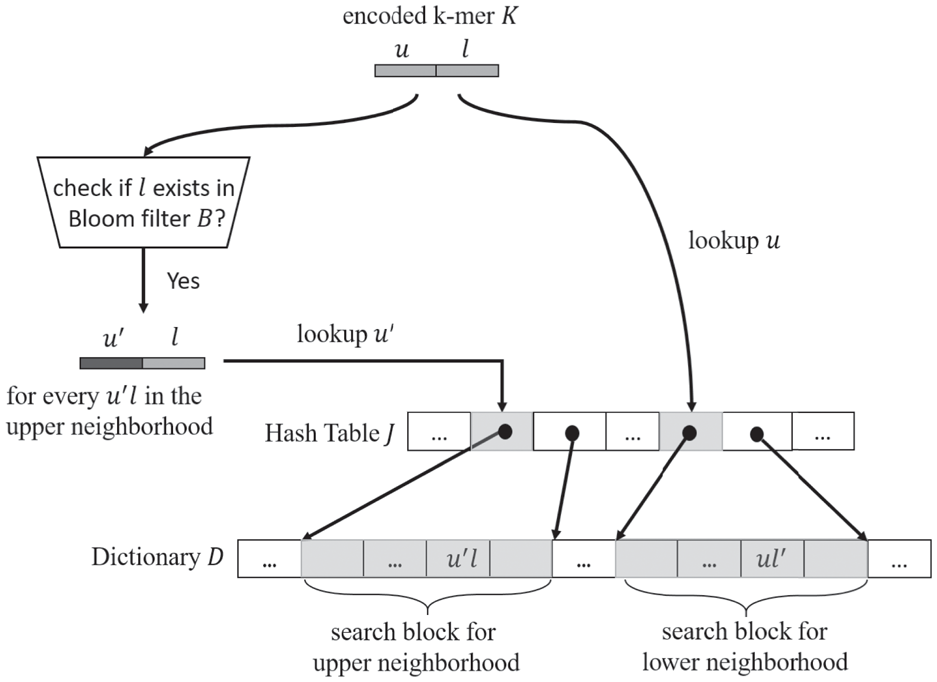
\includegraphics[scale=.40]{images/vargeno-query.png}
  	\caption{Algoritmo di query, VarGeno.}
  	\label{fig:vargeno}
\end{figure}

\paragraph{}
Confrontando i due procedimenti di indicizzazione e di query di LAVA e VarGeno, possiamo ritonare all'affermazione dell’introduzione: il framework VarGeno si basa su LAVA, aggiungendo l’uso del Bloom Filter e la scansione lineare se la dimensione del blocco individuato nel vicinato inferiore ha una dimensione ridotta. Queste euristiche consentono, nella pratica, di migliorare il tempo di esecuzione.

Per le query nel vicinato superiore, ogni k-mer avrà bit superiori diversi e quindi richiederà un accesso separato a \textit{J} e un accesso casuale a \textit{D}. Probabilmente gli accessi a \textit{D}, per ogni k-mer nel vicinato superiore, porteranno a un miss cache, poiché dobbiamo trovare esattamente i (2k - r) bit inferiori. Usando il Bloom filter \textit{B}, proviamo a fare l’accesso solo per i k-mer che rischiano di provocare un match, ed eliminiamo molti accessi inutili e costosi.

Per le query nel vicinato inferiore, l’uso la scansione lineare quando la dimensione del blocco è piccola può comportare un miglioramento significativo delle prestazioni. Sebbene la ricerca binaria sia asintoticamente più veloce, il suo sovraccarico rispetto a una scansione lineare la rende più lenta quando la dimensione del blocco è ridotta: \cite{sun-medvedev2018vargeno} dimostra che il numero di blocchi con dimensione maggiore di \textit{t} è piccolo. 

\textbf{Osservazione.} Dato \textit{n} il numero di k-mer distinti memorizzati nel dizionario \textit{D} e \textit{b} il numero di blocchi, se i k-mer codificati sono indipendenti l'uno dall'altro, la dimensione di un blocco in \textit{D} è almeno \textit{t} con probabilità al massimo $n/bt$. 

Anche se i k-mer codificati non sono indipendenti perché molti si sovrappongono, le posizioni dei blocchi di due k-mer codificati sono molto meno dipendenti.  Questo comporta che, per il genoma umano in cui il numero di k-mer \textit{n} è circa 3 miliardi e \textit{b} è circa $2^{32}$, la probabilità che un blocco sia maggiore di \textit{t} = 25 è $<0,028$. Pertanto, l’algoritmo stima di ricorrere al metodo di ricerca binaria per meno del 3\% dei blocchi: in tutti gli altri casi viene utilizzata la scansione lineare che in questi casi è più veloce.\\

Partendo dall’indice costruito per tutti i k-mei nel genoma di riferimento e dall’indice composto dai k-mer con posizioni che si sovrappongono ad alcuni SNP nella lista SNP con l'allele alternato al posto dell’allele di riferimento, VarGeno prende ciascuna read, la suddivide in k-mer non sovrapposti come LAVA, e interroga i due indici, con il procedimento di query citato precedentemente. In aggiunta, vengono esplorati solo i vicini il cui punteggio di qualità per una determinata posizione è superiore a una soglia \textit{c}, altrimenti essi vengono saltati e non cercati nell’indice, poiché è improbabile avere un errore di sequenziamento in una posizione con un alto punteggio di qualità \cite{sun-medvedev2018vargeno}: questa regola è un’aggiunta rispetto all’algoritmo di LAVA. Di default, VarGeno utilizza \textit{c} = 23, un valore intermedio, per ottenere prestazioni equilibrate.


Dopo aver effettuato le ricerche dei i k-mer da una lettura, VarGeno determina la singola posizione di mappatura per la read. Una read è considerata mappata su una posizione del genoma di riferimento se valgono tutte le seguenti condizioni: (1) quella posizione ha il maggior numero di corrispondenze, (2) almeno due dei k-mer che corrispondono provengono da posizioni diverse della read e (3) almeno un k-mer non deve essere modificato (cioè presente nella read senza una sostituzione); se più di una posizione soddisfa questi criteri la read viene scartata. Un’ulteriore differenza con l’algoritmo di LAVA è in questi tre criteri: LAVA utilizza infatti solo il primo. Decisa la posizione di corrispondenza migliore della read sul genoma di riferimento, la read viene utilizzata per supportare l'allele di riferimento o l’allele alterato degli SNP all'interno della posizione corrispondente. Le informazioni sono memorizzate in una ‘pileup table’ che poi, con lo stesso modello probabilistico di LAVA, usando il teorema di Bayes, determina il genotipo più probabile per ciascun SNP nella lista.

\subsubsection{Prestazioni}
\cite{sun-medvedev2018vargeno}, presentando il loro framework effettuano quindi dei test per verificare i relativi miglioramenti ottenuti, utilizzando più liste di SNP, confrontando prestazioni, tempi e accuratezza del loro framework rispetto a LAVA ed altri algoritmi basati sull’allineamento. LAVA effettuava la genotipizzazione in un tempo molto inferiore ai più comuni algoritmi basati sull’allineamento delle read, perciò anche VarGeno, che si porpone come un'evoluzione di LAVA, ottiene tempi molto inferiori ad essi: VarGeno è 62 volte più veloce dell’algoritmo BWA+mpileup (basato sull'allineamento), con accurancy paragonabile. 

Il punto debole di questi algoritmi che non utilizzano l’allineamento è la memoria richiesta, che è elevata, per mantenere gli indici. VarGeno infatti richiede circa 60 GB nell’esperimento in cui si utilizza la lista dbSNP e circa 44 GB con l’ Affymetrix SNP list. Viene presentata di conseguenza, una versione lite, chiamata VarGeno \textit{Lite}, in grado di diminuire la memoria usata poiché, invece di includere ogni k-mer del genoma di riferimento nell'indice, vengono inseriti solo i k-mer che si trovano all'interno di un intervallo di lunghezza di una read di un SNP nella lista SNP. In questo modo, per la lista dbSNP la memoria viene ridotta del 44\% e del 64\% per l’Affymetrix SNP list.\\


Per quanto riguarda il confronto diretto con LAVA, rispetto al dataset dbSNP, VarGeno è 7-13 volte più veloce di LAVA su tutti i dataset di riferimento usati. L'utilizzo della memoria, la parte debole dei framework, è dominato dalla dimensione degli indici ed è maggiore del 2\% per VarGeno rispetto a LAVA; 'accuratezza di VarGeno è 2-3 punti percentuali superiore a quella di LAVA, grazie all’uso della soglia di qualità \textit{c} e dei criteri di mappatura aggiunti. 

Un dato interessante concerne il miglioramento ricavato dal solo utilizzo del Bloom filter: aggiungendo solo questo componente all’algoritmo di base di LAVA, per quanto riguarda il test riportato da \cite{sun-medvedev2018vargeno}, il tempo viene ridotto del 46\% poiché viene ridotto il numero di cache miss, alle spese solo di un incremento del 2\% di memoria. Aggiungendo invece solo l’ottimizzazione della scansione lineare all’algoritmo di base di LAVA comporta un miglioramento del 38,5\% del tempo di esecuzione. 

Per concludere, analizziamo l’effetto del valore della soglia di qualità: VarGeno non genera vicini in posizioni con punteggio di qualità più della soglia \textit{c}. Al variare di \textit{c}, si osserva un compromesso tra tempo di esecuzione e precisione: la massima precisione viene raggiunta con \textit{c} = 42, che equivale a disabilitare il valore soglia di qualità e generare tutti i vicini di Hamming, mentre il tempo di esecuzione più veloce si ottiene a \textit{c} = 0, che equivale a non esplorare nessuno dei vicini. Si osserva poi un compromesso tra recupero e precisione: con \textit{c} = 42 si ottiene il recupero più elevato e \textit{c} = 0 la massima precisione, con il numero maggiore di identificazioni corrette; in tutti i casi, VarGeno è più veloce e più preciso di LAVA. 


\end{document}